\documentclass[10pt, twocolumn]{article}
%\pagestyle{plain}

\usepackage{amsfonts}
\usepackage{graphicx}


% This is how to make a comment

% These set the margins on your pages
%\hoffset=-1in
%\textwidth=6.5in
%\topmargin=0in
%\voffset=-0.75in
%\textheight=10in

\begin{document}



\title{SimHash: Hash-based Similarity Detection}

\author{Caitlin Sadowski\\
University of California, Santa Cruz\\
supertri@cs.ucsc.edu\\
\and
Greg Levin\\
University of California, Santa Cruz\\
glevin@cs.ucsc.edu}


%\date{}
\def\copyrightspace{}

\maketitle

\section{Abstract}

Most hash functions are used to separate and obscure data, so that similar data hashes to very different keys.  We propose to use hash functions for the opposite purpose: to detect similarities between data. 

Detecting similar files and classifying documents is a well-studied problem, but typically involves complex heuristics and/or $O(n^2)$ pair-wise comparisons. Using a hash function that hashed similar files to similar values, file similarity could be determined simply by comparing pre-sorted hash key values.  The challenge is to find a similarity hash that minimizes false positives. 

We have implemented a family of similarity hash functions with this intent.  We have further enhanced their performance by storing the auxiliary data used to compute our hash keys.  This data is used as a second filter after a hash key comparison indicates that two files are potentially similar.  We use these tests to explore the notion of ``similarity.''


\section{Introduction}

As storage capacities become larger it is increasingly difficult to organize and manage growing file systems. Identical copies or older versions of files often become separated and scattered across a directory structure. Consolidating or removing multiple versions of a file becomes desirable. However, deduplication technologies do not extend well to the case where files are not identical. Techniques for identifying similar files could also be useful for classification purposes and as an aid to search.  A standard technique in similarity detection is to map features of a file into some high-dimensional space, and then use distance within this space as a measure of similarity.  Unfortunately, this typically involves computing the distance between all pairs of files, which leads to $O(n^2)$ similarity detection algorithms.  If these file-to-vector mappings could be reduced to a one-dimensional space, then the data points could be sorted in $O(n \log n)$ time, greatly increasing detection speed.

Our goal was to create a ``similarity hash function.''  Typically, hash functions are designed to minimize collisions (where two different inputs map to the same key value).  With cryptographic hash functions, collisions should be nearly impossible, and nearly identical data should hash to very different keys.  Our similarity hash function has the opposite intent: very similar files should map to very similar, or even the same, hash key, and distance between keys should be some measure of the difference between files.  Of course, ``file size'' is a sort of hash function on files which satisfies these requirements.  However, while similar files are expected to have similar sizes, there is no expectation that two files which are close in size have similar content.  It is necessary to minimize the number of such ``false positives'' in similarity hashes in order to implement a practical system.  However, it is not at all clear how to condense information from a file into a more useful one-dimensional key.

While SimHash does produce integer-valued hash keys, we ended up relying on auxiliary data to refine our similarity tests.  Our key values are based on counting the occurrences of certain binary strings within a file, and combining these sums.  Unfortunately, the key values still end up being roughly proportional to file size, causing many false positives.  However, the auxiliary data provides an easy and efficient means of refining our similarity detection.  A refined version of our keys based on file extension gives a much wider spread of key values, and alleviates some of the aforementioned problems.


\section{Semantics of Similarity}

``Similarity'' is a vague word, and can have numerous meanings in the context of computer files. We take the view that in order for two files to be similar they must share content. However, there are different ways to define that sharing, or what is meant by ``content.'' Take a text file encoded in RTF format as an example. Content could refer to the entire file, just the text portion of the file (not including RTF header information), or the semantic meaning of the text portion of the file (irrespective of the actual text). 

Many previous attempts at file similarity detection have focused on detecting similarity on the \emph{text} \cite{hpDocRepositories, hoad} level. We decided to use \emph{binary} similarity as our metric. Two files are similar if only a small percentage of their raw bit patterns are different. This often fails to detect other types of similarity.  For example, adding a line to source code file might shift all line numbers within the compiled code.  The two source files would be detected as similar under our metric; the compiled results would not.  However, we decided on binary similarity because we did not want to focus on one particular file type (e.g. text documents) or structure. 

Another issue we do not explore is that of semantic similarity. For example, two text files may use different words but contain the same content in terms of meaning. Or, two MP3 files of the same song with different encodings may result in completely different binary content.  We focus on syntactic, not semantic, similarity. In the words of Udi Manber, ``we make no effort to \emph{understand} the contents of the files.'' \cite{manber}

Broder \cite{broder} first made clear the distinction between \emph{resemblance} (when two files resemble each other) and \emph{containment} (when one file is contained inside of another). As an example of a containment relationship, take the case where one file consists of repeated copies of another smaller file. The focus of SimHash has been on resemblance detection. Two files with a significant size disparity (as in the example above) are implicitly different; containment relationships between files do not necessarily make two files 'similar' under our metric.

In order for files to be similar under our estimation, they must contain a large number of common pieces. Another dividing point of techniques is the granularity and coverage of these pieces. SimHash operates at a very fine granularity, specifically byte or word level. We do not attempt complete coverage; we only care about the portions of the file which match our set of bit patterns.

Given some similarity metric, there needs to be a threshold to determine how close within that metric files need to be to count as similar. We are focused on files which have a strong degree of similarity, ideally within 1-2\% of each other.

Another issue is whether a form of similarity detection is meant to operate on a relative or absolute level. In other words, is the focus retrieving a set of files similar to a given file, or retrieving \emph{all} pairs of similar files. SimHash does both.


\section{Implementation}

Our hash key is based on counting the occurrances of certain binary strings within a file.  The keys, along with certain intermediate data, are stored in a relational database (Figure \ref{processingFiles}).  A separate program then queries the database for keys with similar values, and outputs the results.  The particulars of our method are described below.  Our code was written in C++, and developed simultaneously for the Windows and Macintosh platforms. While the code runs equally well on both platforms, we used a Windows machine for primary development and a Mac for most data collection.

 \begin{figure}[h] 
 \centering
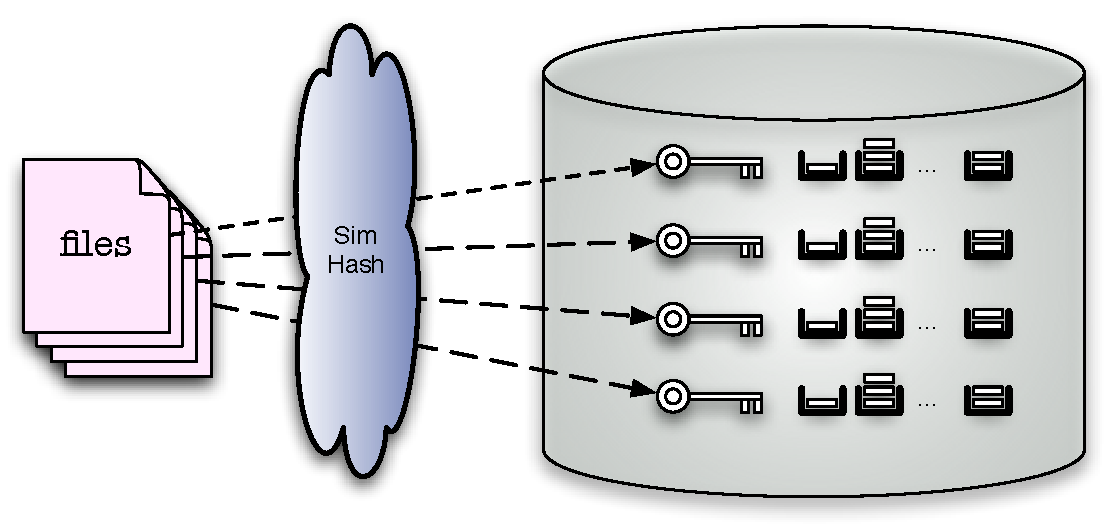
\includegraphics[width= 3in]{processFile.pdf}
\caption{SimHash processes files on a per-directory basis and stores the hash keys and sum table values in a relational database.}
\label{processingFiles} 
\end{figure}   

\subsection{Computing Hash Keys}

Since our notion of similarity is based on binary similarity, we start by counting the occurrances of various binary strings within the file being processed.  We preselect a set of strings, called {\it tags}, to search for.  We only use a subset of all possible strings of a given length, as summing matches over all strings would blur file differences and essentially only return file size.  String size was important, since shorter strings would not represent meaningful patterns, and longer strings would not be expected to occur with meaningful frequency in smaller files.  We chose to use 16 8-bit tags, although we experimented with several different tag sets.

Our {\tt SimHash} program (Figure \ref{simHash}) opens each file in a directory, scans through it, and looks for matches with each of our tags.  We decided to advance our detection window one bit at a time, rather than one byte, since bit patterns across consecutive bytes encode some small information about byte order.  This also gives us a larger and more varied key space, which allows more refined similarity detection.  When a match is found, a skip counter is set and then decremented in the following bits.  This prevents overlaps of matches on the same tag (for example, {\tt 0x00} will only be detected twice, and not 9 times, when two consecutive zero bytes are scanned).  A count of matches, or {\it hits}, is kept for each tag, and these are stored in a {\it sum table}.  The hash key is then computed as a function of the sum table entries.  We restrict our attention to linear combinations of the sums, as giving an order of magnitude more weight to one tag over another would be basically equivalent to not using the other tag at all.  However, we did experiment with various weighting schemes within our linear combinations.  Once this has all been computed, the file name, path, and size, along with its key and all entries in the sum table, are stored in  a MySQL database.  Later on, we added the capacity to compute and store multiple keys per field, so that different sum table weightings could be compared side-by-side, or used as additional filters.

 \begin{figure}[t] 
 \centering
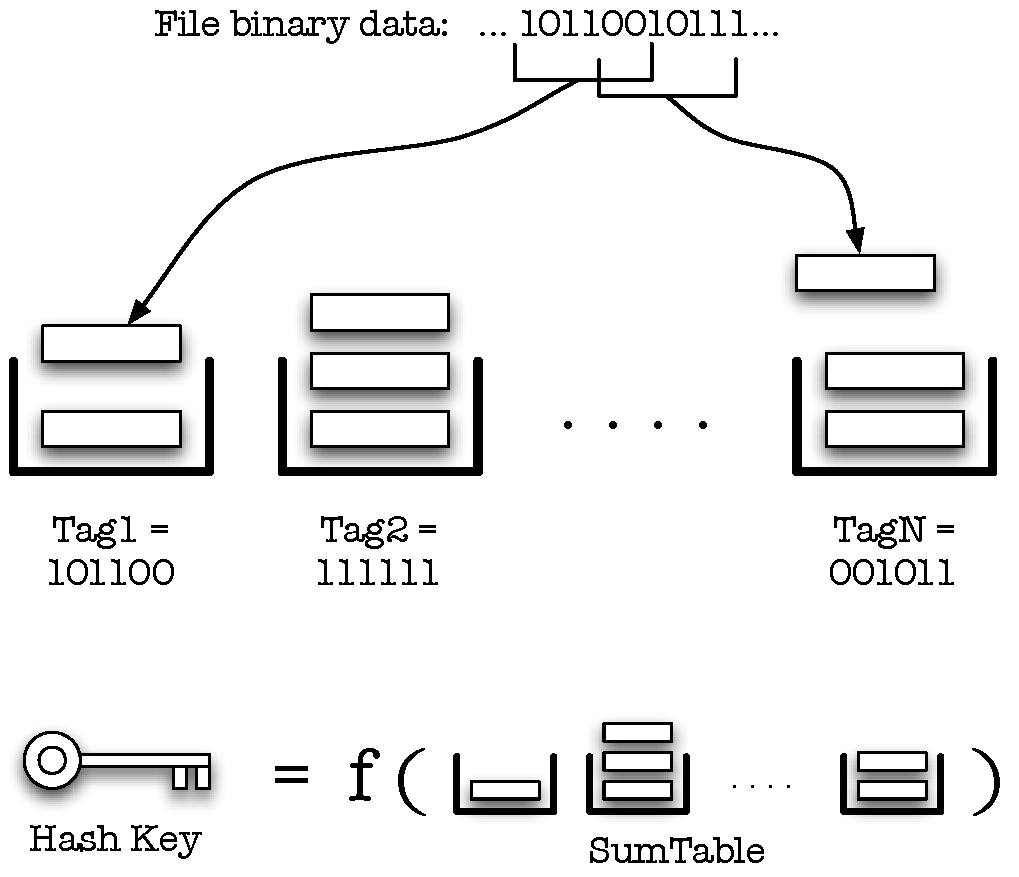
\includegraphics[width= 3in]{simHashInternals.pdf}
\caption{SimHash produces two levels of file similarity data: tag counts make up the sum table entries, which are then combined to form a hash key.}
\label{simHash} 
\end{figure}   

A variation of the key function was implemented to account for file extensions.  It is not unreasonable to claim that two files are inherently different if they have different extensions.  Given this, it would be desirable for our hash function to assign very different values to any two files with different extensions.  To this end, we compute a simple hash of (the first three characters of) a file's extension, with a value between 0 and 1.  The distribution of these values should be fairly uniform across the space of possible extensions.  We then multiply this extension value by {\tt MAX\_INT}, and add that to our previous key value.  Since we only care about the {\it distance} between keys, and not their actual values, this will not affect the relation between files with the same extension, while it will tend to widely separate files of different extensions.  This has the effect of more evenly distributing our key values across the space of 32-bit integers, and making cross-extension key matches very unlikely.

 \begin{figure}[h] 
 \centering
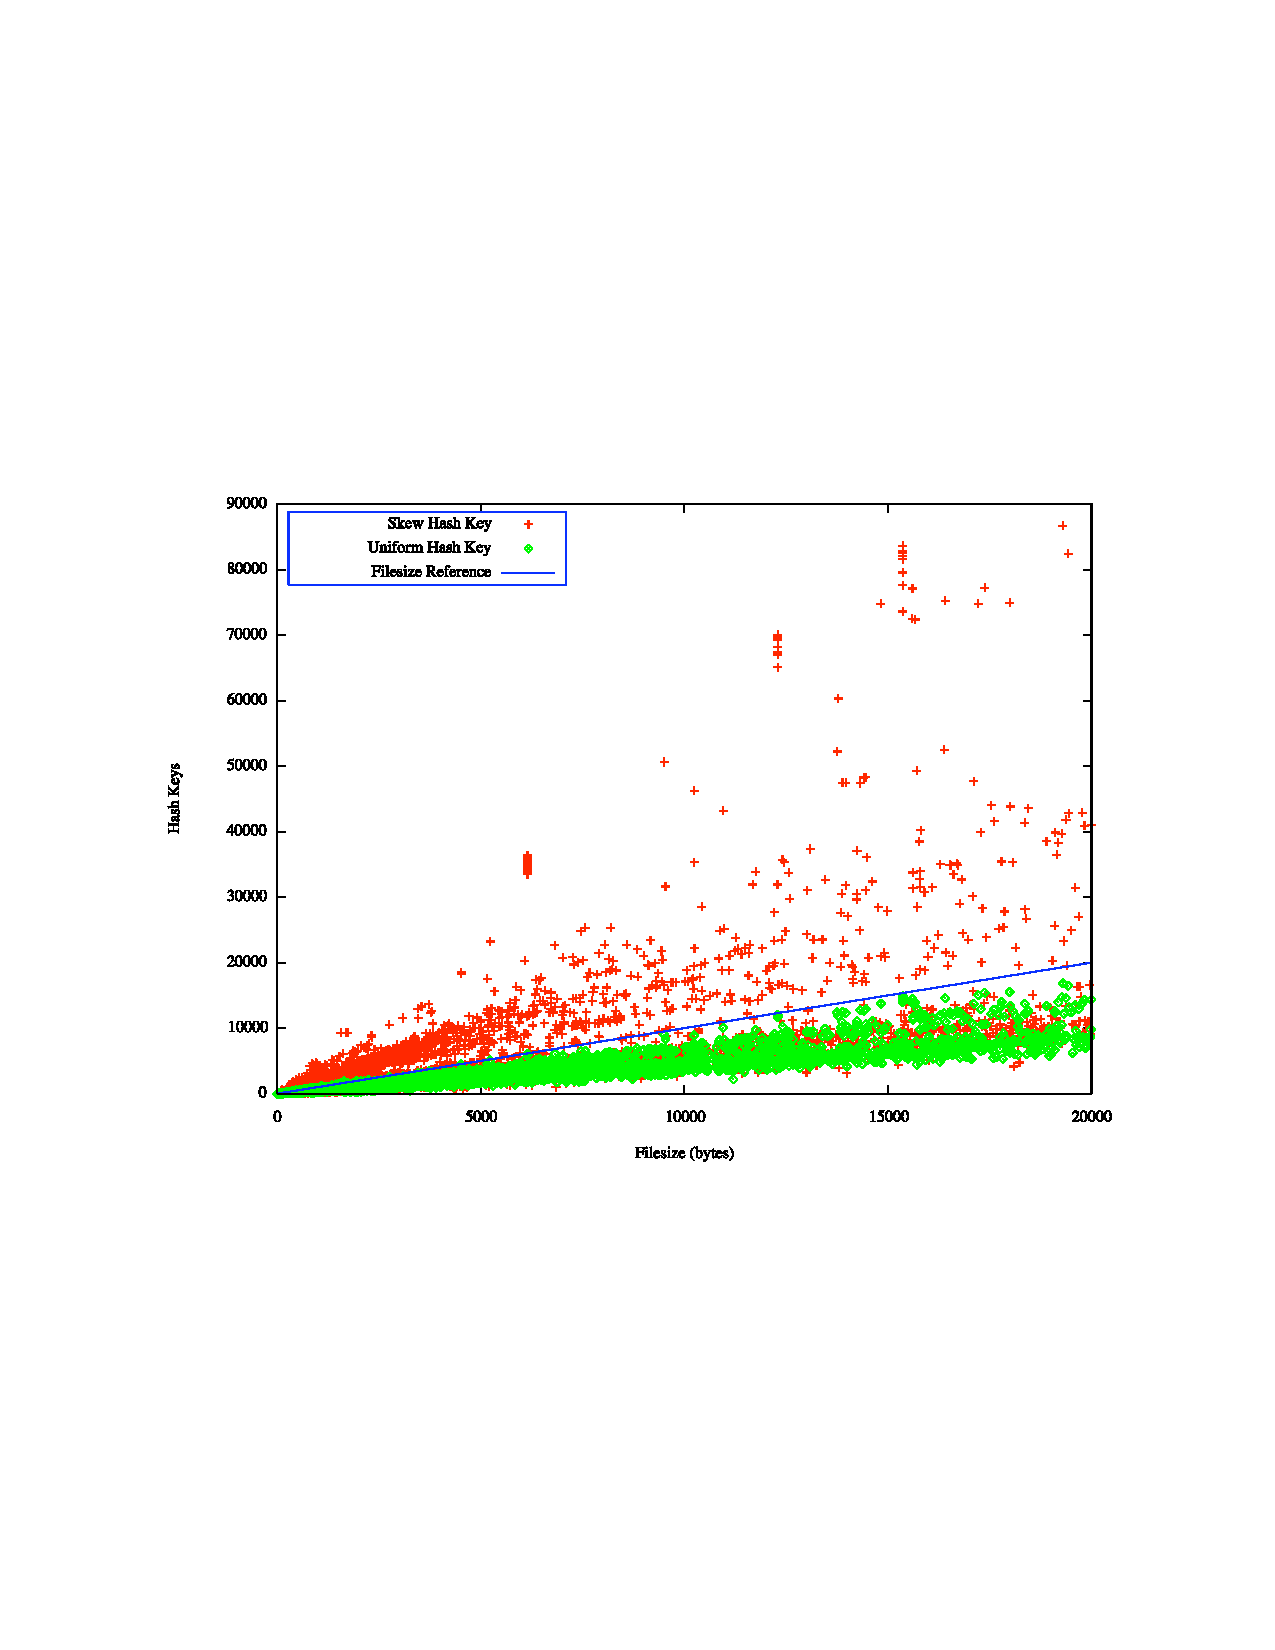
\includegraphics[width= 3in]{scatter_circles.pdf}
\caption{Visualization of Key Spaces for Uniform and Skew Keys}
\label{scatterPoster} 
\end{figure}   

 \begin{figure}[h] 
 \centering
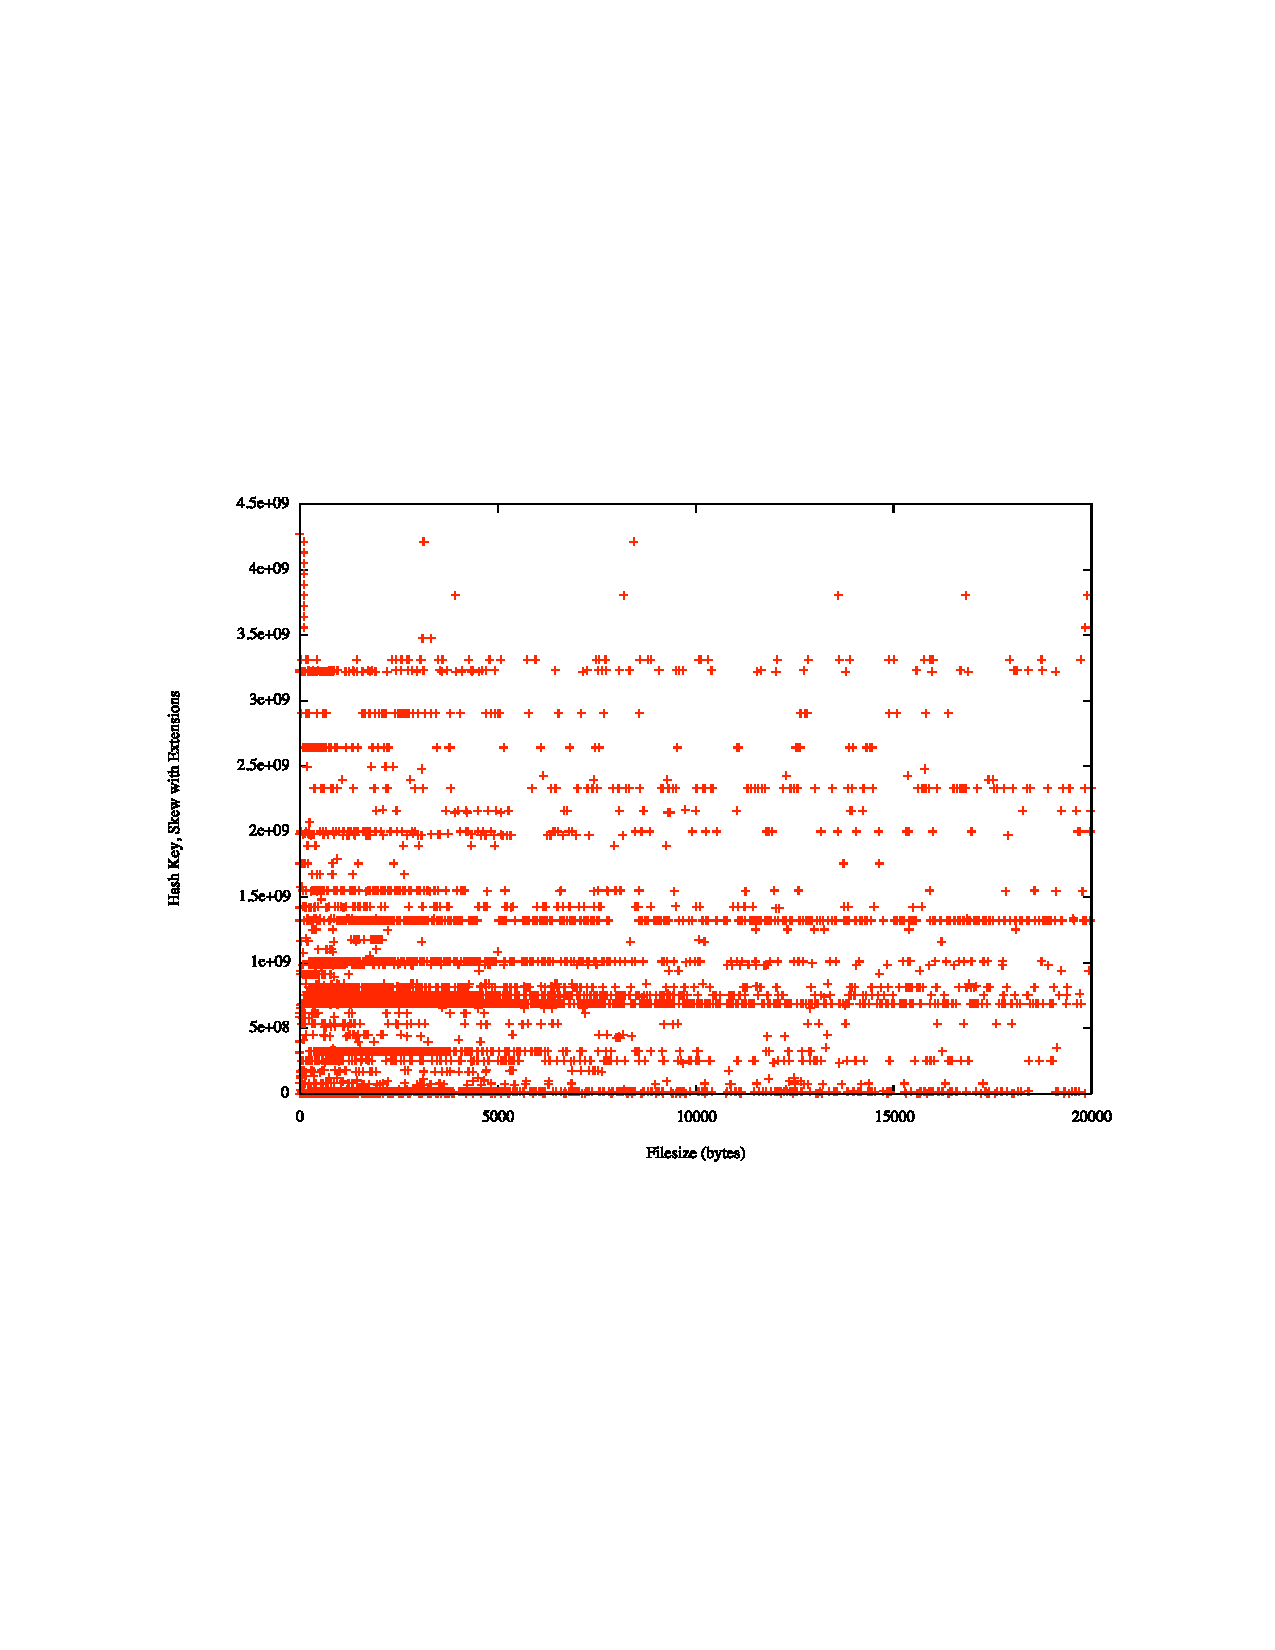
\includegraphics[width= 3in]{skewExtScatter.pdf}
\caption{Visualization of  Skew Key Space with File Extension Modification}
\label{scatterExtension} 
\end{figure}   

Figures \ref{scatterPoster} and \ref{scatterExtension} are visualizations of various key spaces, with key values plotted against file sizes.  Figure \ref{scatterPoster} shows the key spaces for keys with identical weights (Uniform) and heavily imbalanced weights (Skew), and plots the line $y=x$ for reference.  Note that both key values are roughly proportional to file size, although the Skew Key has a wider variance.  Figure \ref{scatterExtension} shows the Skew Key with file extension modification.  Keys span the full range of 32-bit values, with horizontal stripes representing different file extensions.  It is clear from the picture that key hits between different file types would be highly unusual.  For further discussion of these keys, see Section 5.



\subsection{Finding Similarities}

Once the database has been populated with the data from a test directory, we use a second program called {\tt SimFind} to look for similar keys (Figure \ref{simFind}).  One file at a time, we perform a SQL query on its key to find all other key values within a certain tolerance range.  We set a single tolerance level across all files, and then multiply this value by the size of our target file, since we expect key values to increase proportionally to file size.  This is only the first level of our similarity filter.  For each file returned in this query, we first discard it if the file size differs too much from our first file.  Next, we compute the distance between their sum tables, which is just the sum of the absolute values of the differences between their entries.  If this distance is within a certain tolerance (proportional to the key tolerance and file sizes), then we report the two files as similar.  Further, if the sum table distance is zero, the two files are compared directly to determine if they are, in fact, identical files.

 \begin{figure}[h] 
 \centering
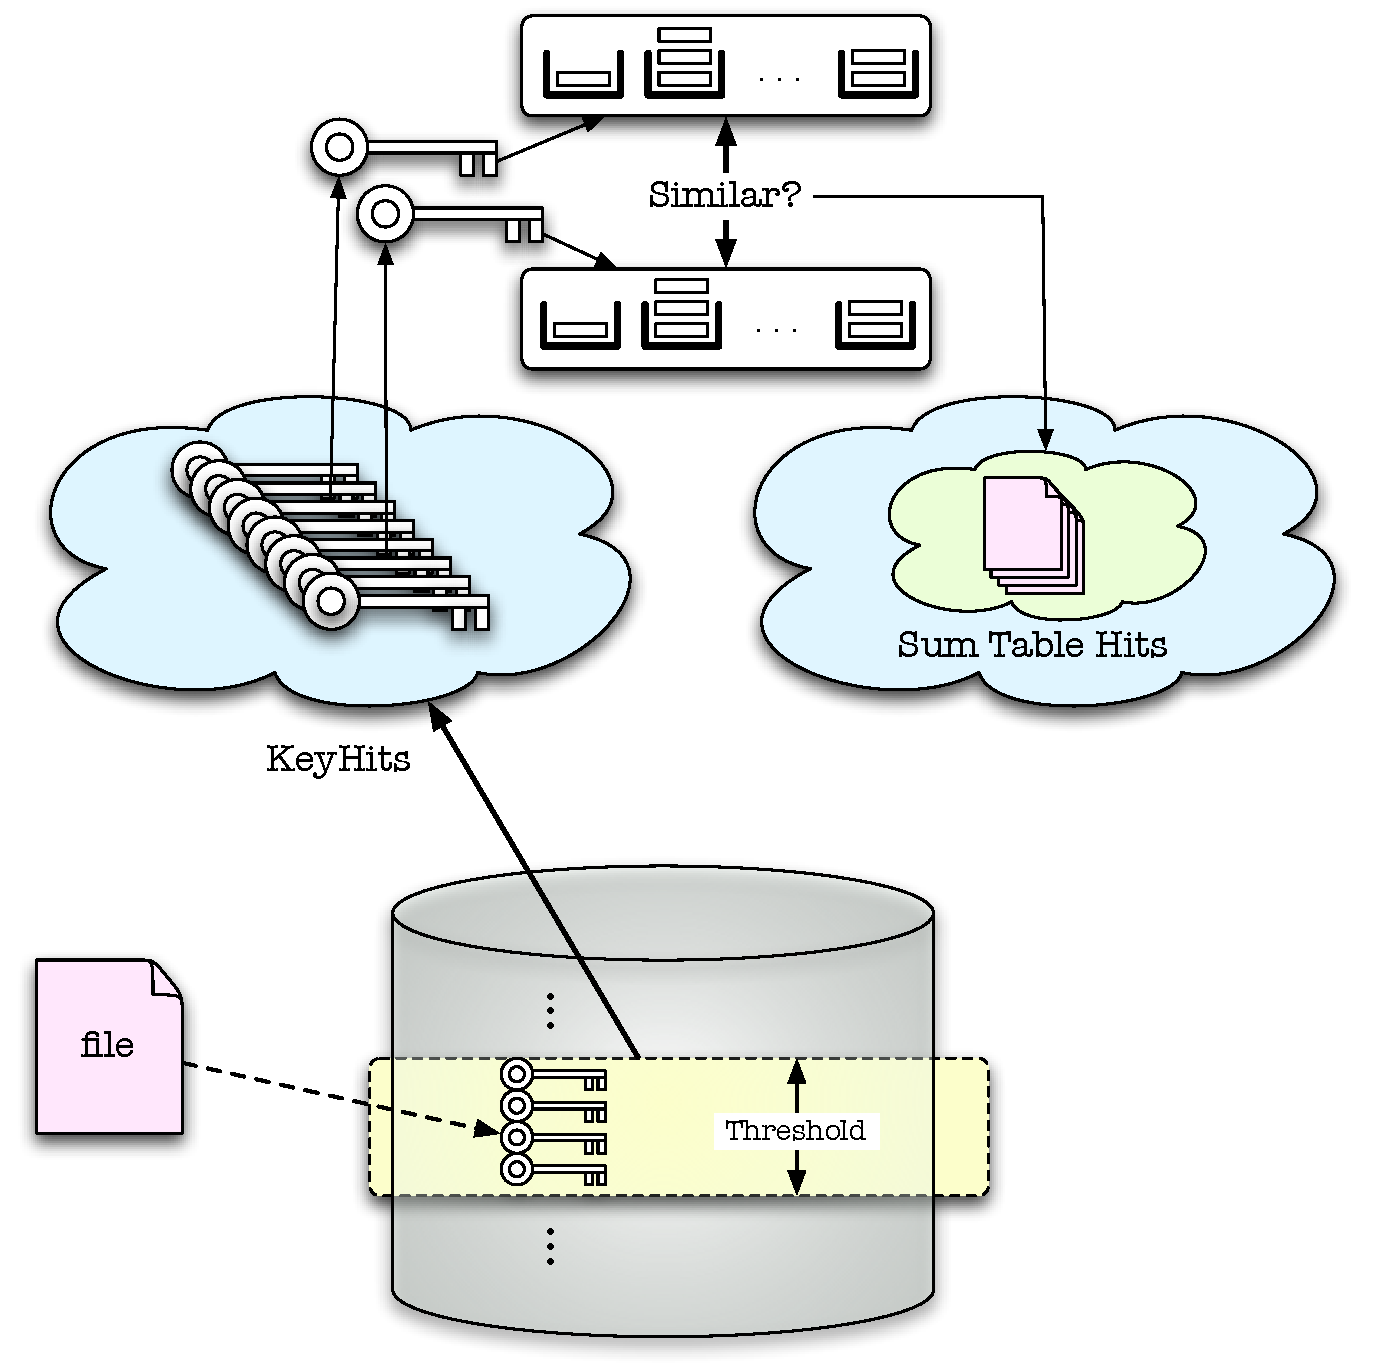
\includegraphics[width= 3in]{simFind.pdf}
\caption{SimFind identifies all files which have key values within a certain tolerance of a particular file, then performs pairwise comparisons among the sum table entries to return a filtered selection of similar files.}
\label{simFind} 
\end{figure}   

Essentially, two files are deemed similar if they contain a very similar number of each of our selected tags in their bit patterns.  This method has several strengths and drawbacks.  Because the ordering of the tag matches within a file is not accounted for, rearranging the contents of a file will, up to a point, have little impact on key values and sum tables.  Similarly, adding or removing small pieces of a file will have only a small effect on these values.  Consequently, small changes to a file shouldn't throw off our similarity measure.  Further, the results of our calculations are relatively easy to understand and reason about.  Because ``similarity'' is based on the numerical distance between values, we can easily change the tolerance level for key and sum table distance matches.  Of course, increasing tolerance values both widens the range of similar files found and increases the number of false positives, so a good balance between these must be found.

As the order of strings within files is not measured, very different files can be detected as similar if they happen to share too many bit patterns.  For example, the Law of Large Numbers makes false positives within our key space more likely for large files with effectively random data.  Since key similarity is the comparison that could be theoretically performed with an $O(\log n)$ search through a sorted list, an excess of false positives here means a larger number of pair-wise comparisons that must be performed on our sum table, even if those comparisons are computationally minimal.

\section{Results}

We explored how different selections of tags and tag weights affected our results. We also investigated factoring in other data, such as the file extension, when computing hash keys.  We ran tests on a variety of data sets, both artificially generated and found in the wild. Due to time limitations, we were not able to run as rigorous tests or make as interesting improvements as we would have liked. However, we still gleaned some interesting results.

We found that an unbalanced weighting scheme where only a few tags were used to compute a key worked best on a realistic file set, although a more uniform weighting scheme performed better on contrived data sets. We also identified several problems with our method which highlight areas for future work.

\subsection{Choosing Tags and Keys}

As mentioned above, we settled on 16 8-bit tags to apply our similarity measure.  In trying to select tags, we noticed that {\tt 0x00} was often the most significant single differentiator of file structure.  This is not surprising, as some files are padded with large sections of zeros, while data rich files and text files contain few or no {\tt 0x00} bytes.  Other than {\tt 0x00}, an essentially random selection of bytes values seem to perform generally better than contrived or structured tag sets.  We included the ASCII representations of `e' and `t', as these appeared to be strong indicators of text-based data, and also non-ASCII-range bytes, which would be less prevalent in text files.

We also investigated various relative weightings of tags in the calculation of the hash key.  We tried equal and unequal weightings of all tags, as well as giving zero weights to (i.e. ignoring) a large fraction of our tags.  On the whole, this last scheme performed best on real file sets. One measure of key performance was the ratio of  sum table hits to key hits.  That is, what fraction of key hits are validated as actually similar according to the sum table?  The higher this ratio, the lower the presumed false positive rate of the key.  We also included comparisons using the file extension modification to keys.  Figure \ref{simdiff} shows results of comparing four keys on two distinct file sets.  The Uniform Key has all 16 tags weighted equally, while the Skew Key applies uneven weights to only 4 of the tags, with the {\tt 0x00} tag getting the largest weight (other weighting schemes were tested, but were found to regularly lie between these two extremes).  The ``Similar Files'' set contains a sequence of 4K files, each of which differs in only a few bytes from its predecessor.  Consequently, ``nearby'' files should all be considered similar.  The ``Different Files'' set contains a sample of assorted files from a real file system.  From this set, files with apparent similarities were removed, and all files were truncated to 4K to make results more easily comparable.  That we observe a smaller rate of false positives on a set of similar files is not surprising, since there are simply fewer dissimilar files.  For the somewhat more realistic set of different files, the Skew Key shows better performance\footnote{Note that these are ratios, not absolute counts of similarity hits.  While some effort was made to remove similar files from the ``Different Files'' set, the remaining hits that {\it were} found were all between files with matching extensions, even without the file extension enhancement in place.  Further, matches appeared to occur on genuinely similar files, with similarity decreasing as tolerance increased.}.  Running tests on several other data sets confirmed this observation and so the Skew Key was adopted as the standard key for future tests.

 \begin{figure}[t] 
 \centering
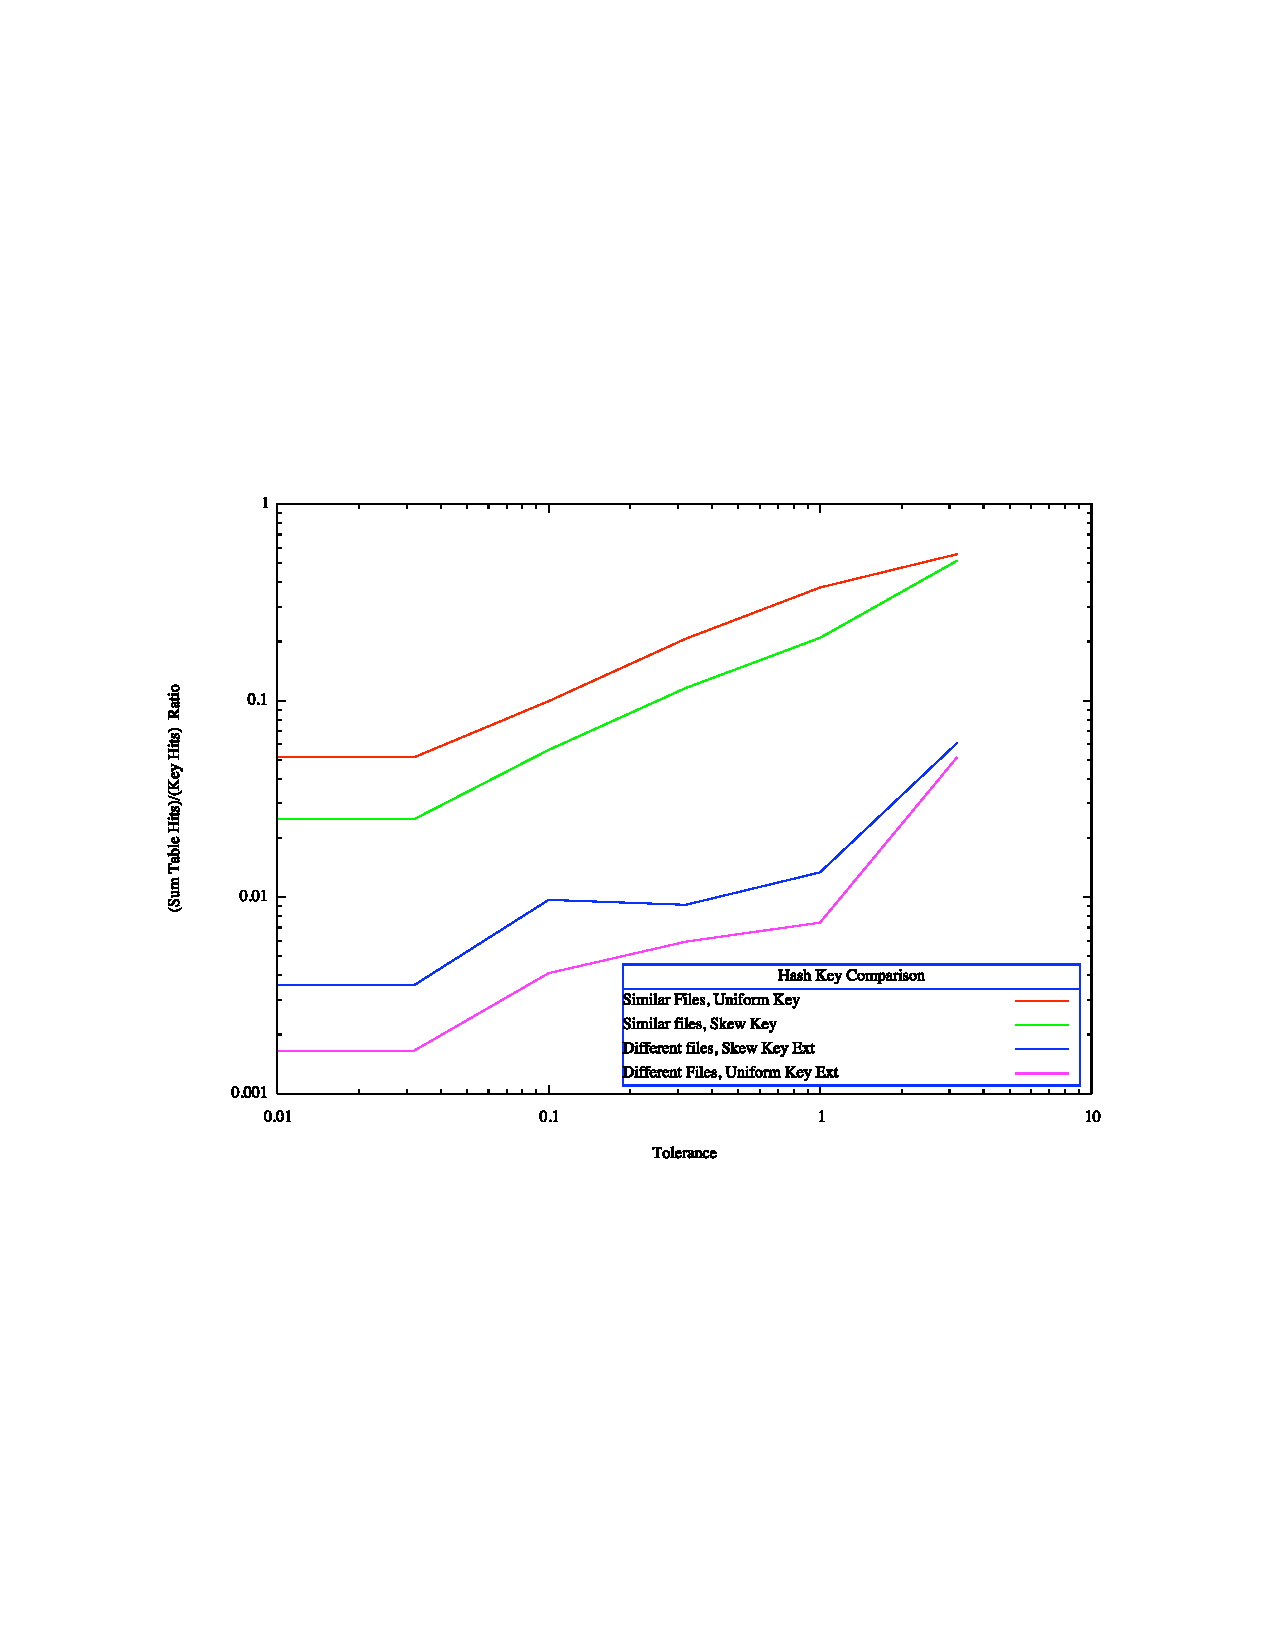
\includegraphics[width= 3in]{ratioSimDiff.pdf}
\caption{Comparing effectiveness of different key strategies on sets of predominantly similar and predominately different files.}
\label{simdiff} 
\end{figure}   

The next trial demonstrated the value of the file extension key modification.  Figure \ref{PairwiseSavings} shows key hits and sum table hits for the Skew Key, with and without the file extension modification.  The trial was run on 10,364 files from a random selection of directories on an existing Macintosh file system.  To normalize the results, values were divided by $\left( \begin{array}{c} n \\ 2 \end{array} \right)$, the total number of pairs of files across the test set.  Even at a rather high tolerance, the Skew Key with extensions is only reporting a match for about one in 5000 pairs, or about two hits per file. In other words, only a small number of auxiliary sum table comparisons are needed on average.  While a file set of 10000 is small compared to an entire file system, the small percentage of matches is an encouraging sign that our methods have some hope of scaling well to larger file sets.

 \begin{figure}[t] 
 \centering
\includegraphics[width= 3in]{PairwiseElim.pdf}
\caption{Number of key and sum table hits with and without the file extension key modification.  Results are scaled by the total number of file pairs in the file set (i.e. ``n choose 2'').  }
\label{PairwiseSavings} 
\end{figure}


\subsection{Problems}

There are a number of problems with our method, although it is not clear if any  generalized similarity measure could address all of these.  One problem we encountered was certain file formats with very large headers.  Postscript is an example of this.  We took 200 randomly generated 4K ASCII files (which should have no more similarity than would be predicted by the averaging effects of the Law of Large Numbers), and then converted them to both PDF and Postscript.  The results of applying the Skew Key to these three sets is shown in Figure \ref{headerFiles}.  In all three formats, there is a critical tolerance region, where we quickly jump from ``none similar'' to ``all similar.''  While the shape of the curves is nearly identical, this threshold appears for Postscript files at a tolerance value nearly 100 times more sensitive than their raw ASCII counterparts.  This is due to common headers and file padding in the more complex file formats.  For example, 4K of raw text translates into a 12K PDF, and an enormous 252K Postscript file.  Obviously, the majority of the file is structure and not content, and so two Postscript files with entirely different data will still show a very high similarity as a percentage of their size.  This makes detecting differences in data problematic for such file formats.  A potential solution would be to manually set the tolerance levels for different file formats.  A very low tolerance setting for Postscript extensions would rule out similarity for differences that amount to only a very small percentage of the file size.

 \begin{figure}[t] 
 \centering
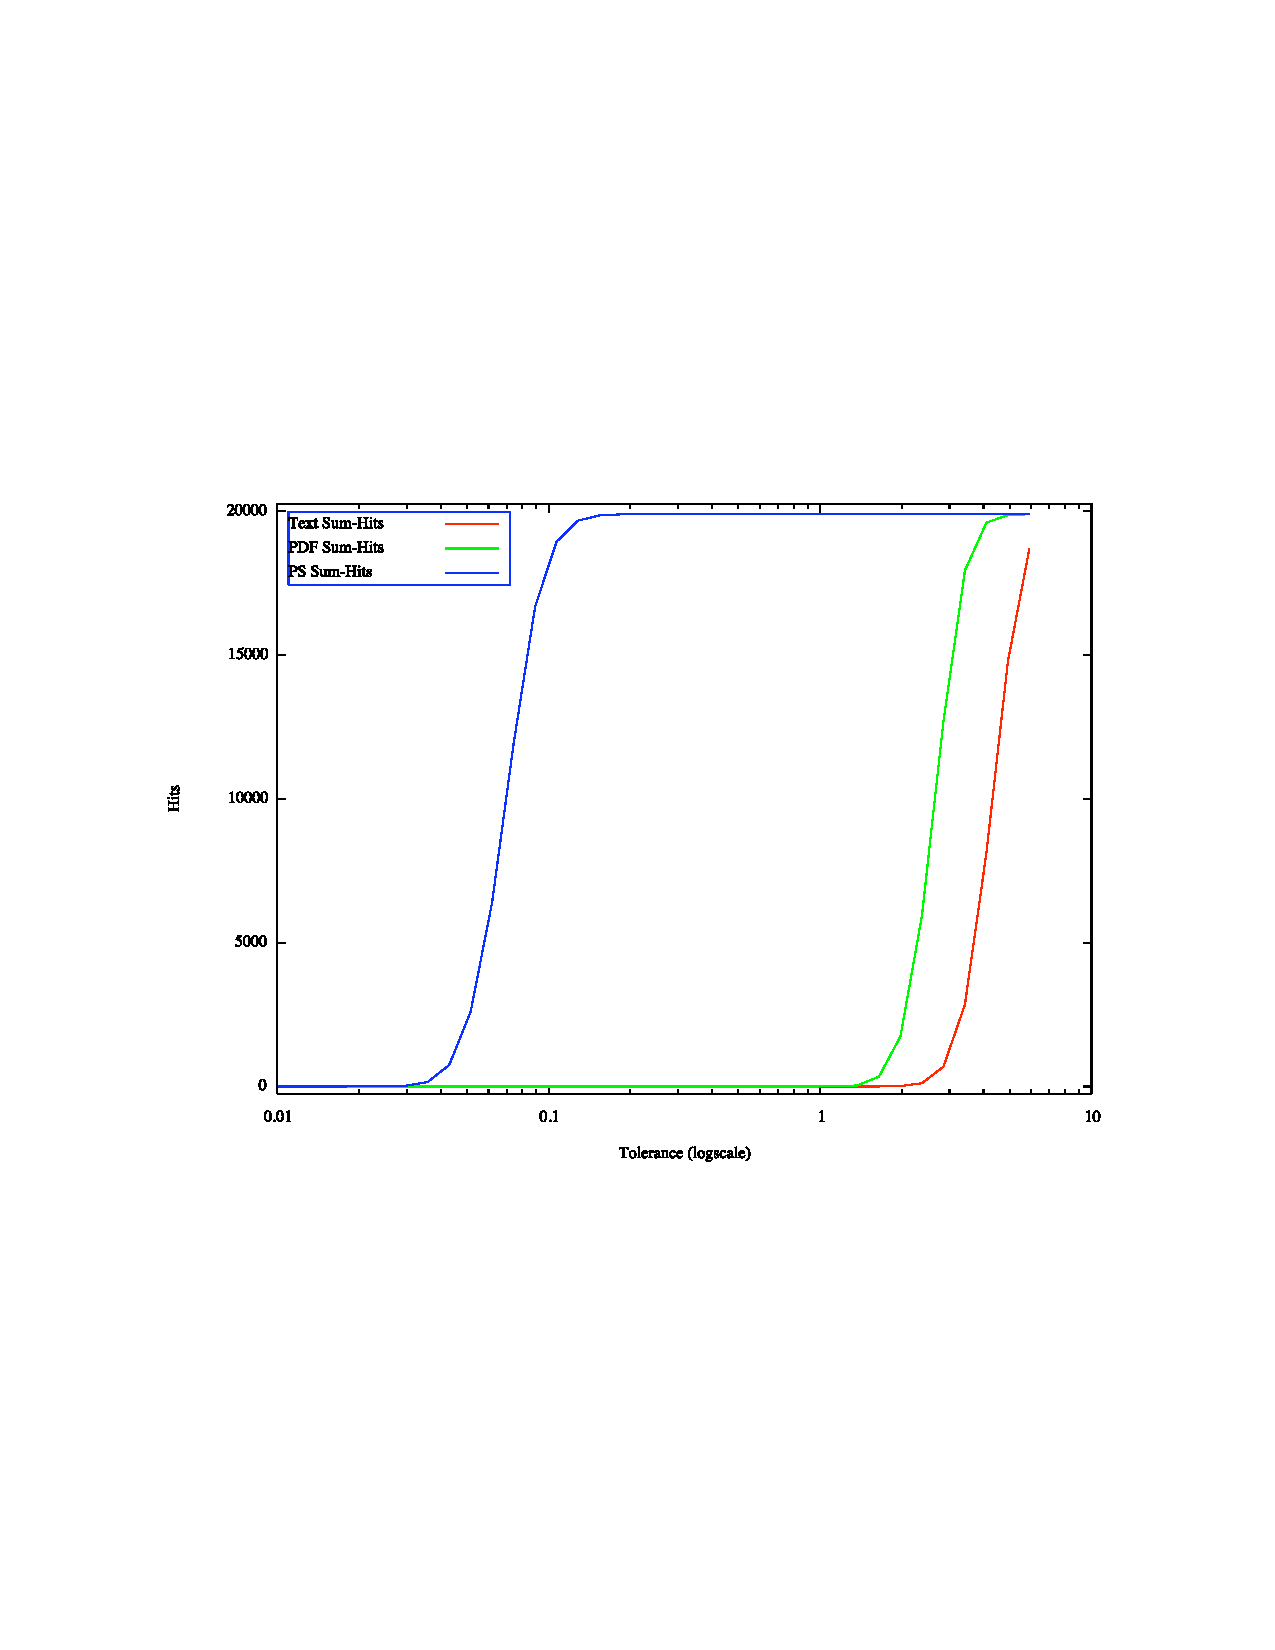
\includegraphics[width= 3in]{fileFormats.pdf}
\caption{Sum table hits for 200 randomly generated ASCII files, with data converted to PDF and Postscript formats.  Large file headers in Postscript cause the same content to be identified as similar at much lower tolerance levels.}
\label{headerFiles}
\end{figure}

Another problem we haven't addressed well is scale.  Due to time and computing constraints, we have only used a maximum test set of 10000 files.  As the presumed environment for similarity detection would be file systems of potentially millions of files, it is not immediately obvious how well our results scale.  In terms of space usage, only a few hundred bytes were necessary to store the SimHash information associated with a particular file. However, in our implementation, most of this was taken up with the file path string for increased readability.  In a more properly integrated implementation, that text could be replaced with the file inode address or other numerical representation, reducing the space usage to approximately 100 bytes per file.

We ran our {\tt SimFind} process on sets of similar files that ranged in count from 500 to 8000, and timed the results.  The results are shown in Figure \ref{performanceTest}.  A quadratic curve is plotted for reference, and our time growth does appear to be $O(n^2)$.  This is exactly the sort of prohibitive growth that the hash key method is intended to avoid, although we must keep in mind that these are sets of very similar files, where numerous key hits are expected.  It should only take $O(\log n)$ time to determine the {\it number} of key matches against a file, but if the number of matches is proportional to the total number of files, then we will need to perform $O(n)$ sum table comparisons for each file.  $O(n^2)$ growth may be unavoidable.  However, within a typical file system, it may be the case that the number of files that actually generate key hits against a single file is a tiny fraction of the overall file count.  If we are lucky, this fraction would be small enough to make the constant on the $O(n^2)$ of a manageable size, so that our method would be still be efficient in practice.  In any case, it was not our expectation that key hits by themselves would provide a reliable measure of fine-grained similarity.  Instead, we expected that they would provide a strong filter which would greatly reduce the number of pair-wise comparisons subsequently needed.

 \begin{figure}[t] 
 \centering
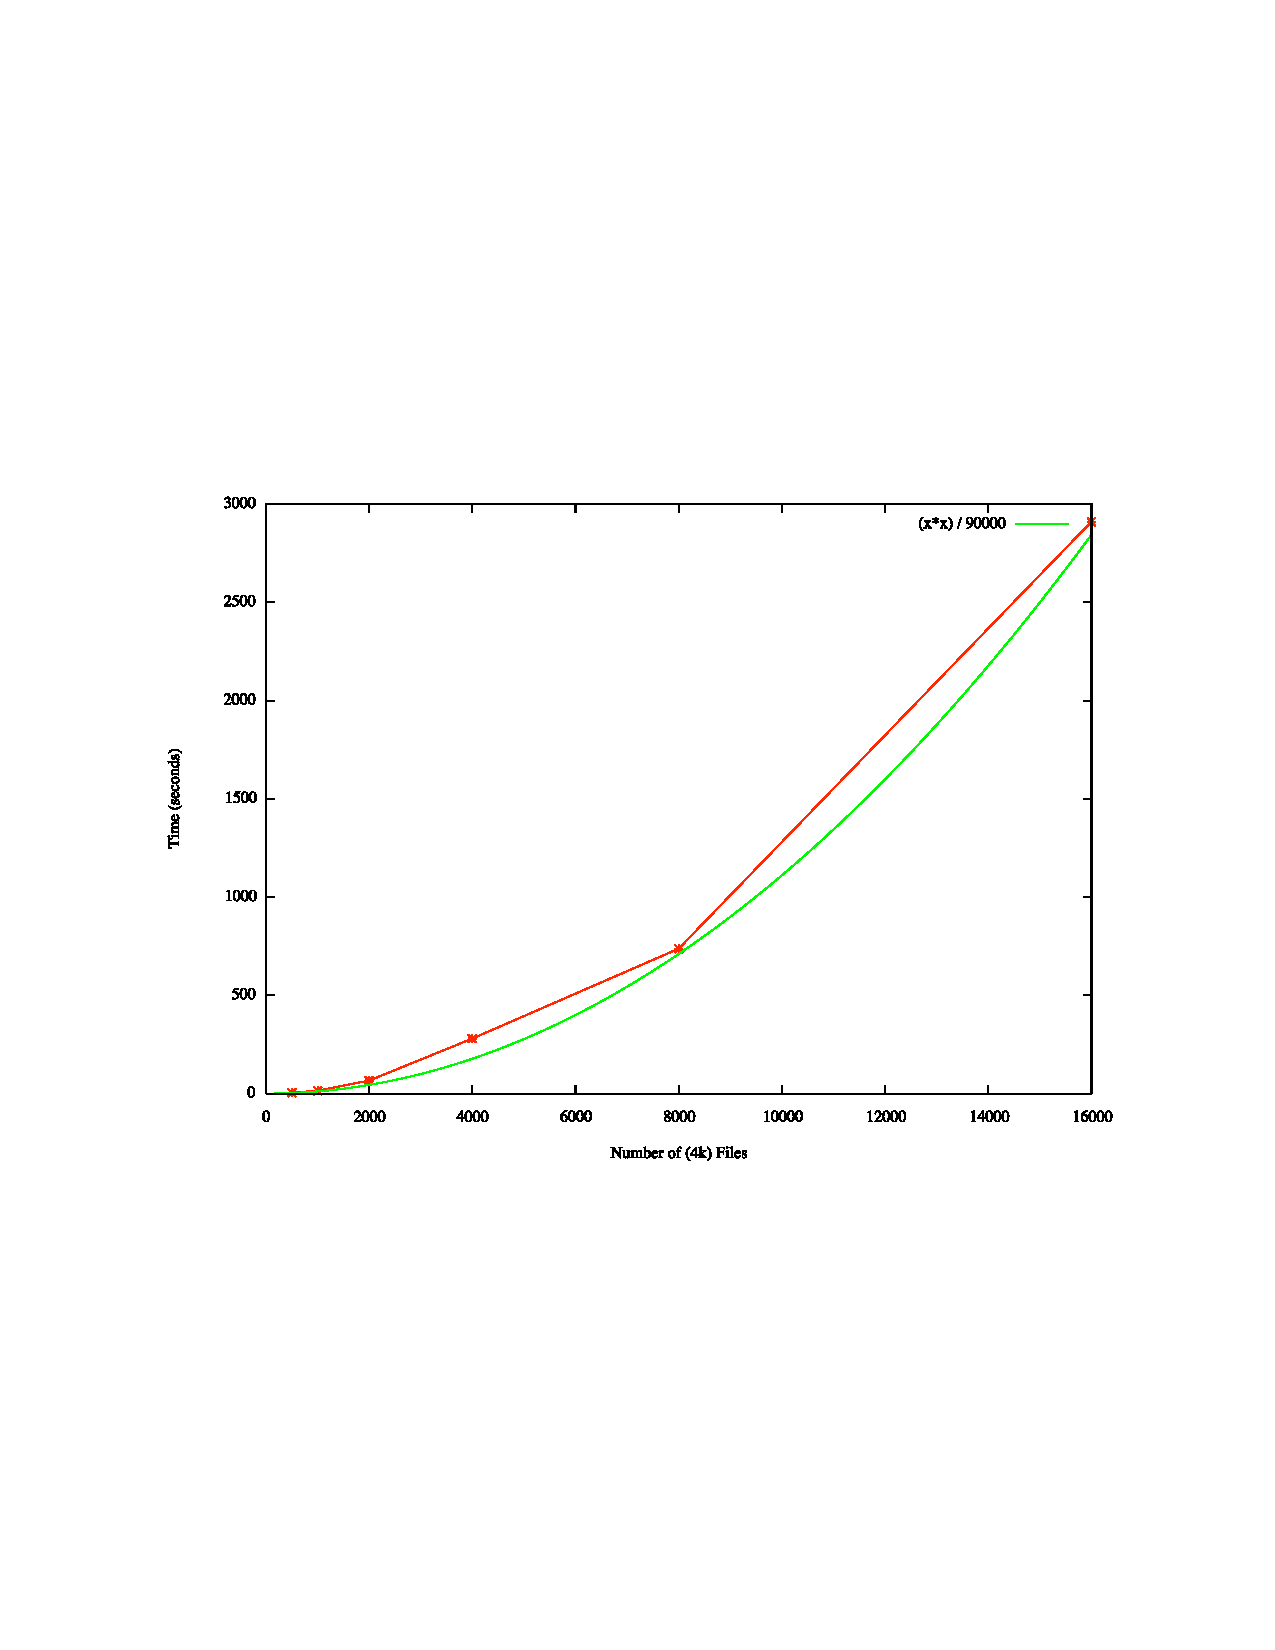
\includegraphics[width= 3in]{performance.pdf}
\caption{Run time versus file count for SimFind on sets of similar files, with a quadratic curve plotted for reference.}
\label{performanceTest}
\end{figure}

A final difficulty that we have not yet come to terms with is the relation between key and sum table hits.  Sum table hits represent a much more accurate measure of similarity.  Ideally, if sum table comparisons would label two files as similar, then those two files should also first pass the courser key similarity test.  In practice, however, this ideal may not be desirable.  Consider the Uniform Key, where all tags are given equal weights.  If two files have a sum table distance of 20, then the differences in their keys would lie somewhere between 0 and 20. If our sum table tolerance is 20, then our key hit tolerance should be 20 as well to allow all possible sum table hits to be checked.  However, only in the extreme case is this high a key tolerance necessary.
%TODO: FIX THIS!
We compared sum table hits to key hits in a data set of similar files made by successively appending bytes to a starter file. In this worst case scenario, the sum hit to key hit ratio approaches one. 

In general, it may be that a key tolerance of 15 only eliminates 10\% of our sum table hits, but reduces the number of false positives by 40\%.  This phenomenon is visible in Figure \ref{PairwiseSavings}, where the improved key with extensions admits fewer sum table hits.  The trade-off for performance vs. accuracy may be acceptable or even desirable.  More work would be required to explore the interaction of these two tolerances, and their actual values could be set based on the needs of a given implementation environment.

\section{Related Work}

The problem of identifying file similarity is not a new one, although no one seems to have discovered a consistently good general solution. The most relevant paper to SimHash is over ten years old \cite{manber}. There has also been a body of research focusing on redundancy elimination or deduplication. Much of the research on similarity detection since then has focused on very specific applications and file types. This includes:
\begin{itemize}
\item technical documentation \cite{hpDocRepositories} 
\item software systems \cite{sourcecode} 
\item plagiarism detection \cite{hoad} \cite{bernstein}
\item music \cite{music}
\item web pages \cite{buttler}
\end{itemize}

In most cases, the main goal of redundancy elimination is a reduction in either bandwidth or storage. Redundancy elimination  can focus on eliminating multiple copies of the same file, or else preventing repeats of specific blocks shared between files. The standard way to identify duplicate blocks is by hashing each block. Venti \cite{venti} is an archival storage system which only stores only one copy of every block. As files are modified, new copies of modified blocks are written to disk, without changing references to unmodified blocks. Shared or unmodified blocks are identified by comparing hashes of the blocks within a file before writing to disk. LBFS \cite{lbfs} exemplifies a similar idea but is focused on bandwidth reduction; when a file is changed, only modified blocks are sent over the network. Redundancy elimination at the block (or chunk) level provides a coarse-grained method of file similarity; files which share enough identical blocks are similar. Forman et al\cite{hpDocRepositories} took this approach when identifying similar documents in a repository. A file is represented by a collection of hashes of content-based chunks. If the collections of a set of files share a large overlap, then the files are considered similar.

A natural question when classifying blocks is how to identify block boundaries. The options for this include fixed size chunking (for example, file system blocks), fixed size chunking over a sliding window (rsync \cite{rsync}), or some form of dynamic content-based chunking \cite{lbfs}. Content-defined chunking consistently outperforms fixed sized chunking at identifying redundancies, but involves larger time and space overheads  \cite{policroniades2004adr}.

Instead of coalescing repeated blocks, delta-encoding works at a finer granularity. Essentially, it uses the difference (or delta) between two files to represent the second one. This is only effective when the two files resemble each other closely.  Different versions in a version control system provide a good example. DERD \cite{derd} investigates dynamically identifying similar files (or web pages) and then using delta-encoding to shrink the total footprint of similar pairs. The goal of REBL \cite{rebl} is heavy redundancy elimination with a combination of previous techniques. Identical and similar (content-based) chunks are identified. Identical chunks are removed, and similar chunks are delta-encoded. The remaining chunks are compressed, which essentially is redundancy elimination within one file.

Udi Manber \cite{manber} developed a technique for finding what he calls \emph{approximate fingerprints} of a file. His approach involves the concept of a set of \emph{anchors}, or small patterns of characters. In each file, a checksum of the characters around occurrences of each anchor is computed. This set of checksums forms the fingerprints for the file, and is compared against fingerprints for other files when searching for similar files. Our sum table counts are in a similar vein. An important distinction between the two ideas is that we also form one hash key for each file.  This serves as a low-cost, first-pass filter which greatly reduces the number of pair-wise comparisons needed.



\section{Future Work}

There are many ways to extend and build on the ideas and methods presented here, some of which were discussed in the results section.  Although it is not immediately clear how, our hash function could almost certainly be improved upon.  Even the file extension modified hash appears to cover only a small portion of our 32-bit key space.  A hash function which covered this space more uniformly while still encoding similarity could provide a much lower rate of false positive key hits.  We could also combine multiple hash keys in a progressive filtering scheme to remove more false positives before getting to the level of sum table comparisons.  Even the sum table pair-wise comparison scheme could be used as an intermediate filter for more complex pair-wise comparison schemes.  Since computing sum table differences is fast and efficient, it might provide an efficiency boost to other methods.  Alternately, we could try to somehow combine our similarity measurements with others.

There are other metrics besides binary similarity which would extend to the diversity of file types available in a system. One other example is metadata about files. We did not use file metadata (author, creation date, etc.) for file similarity detection because we wanted our code to be cross-platform compatible. We also did not want to get caught up with issues of metadata reliability, and so limited our focus to the actual contents of the file. However, one could imagine adding heuristics for metadata similarity to the mix. 

Multiple similarity metrics for different file types could be combined to have a cohesive file similarity measure for the entire system.  Extending SimHash to provide varying built-in tolerance levels for different extensions may alleviate this problem somewhat, but there will still be some file types for which binary similarity does not work (like music files).  As an alternative, SimHash could be made more effective by running certain files through a filter before computing their hash values.  For example, many different document formats are often essentially just text (the aforementioned Postscript, PDF, and RTF, as well as MS Word documents, HTML files, etc).  If the text content were extracted from such files\footnote{Windows provides a generic interface called an {\it ifilter} which does just this for most common file types, and which is supported by vendors of proprietary formats, like Adobe for PDF}, and only the raw ASCII were hashed, then we could come closer to comparing the {\it semantics} of a file, rather than just its raw structure.

Other, more far-reaching schemes can be imagined.  Using the LBFS \cite{lbfs} scheme for dynamically partitioning files into chunks, we could restrict our attention to a similarity hash on file chunks.  One of the main drawbacks of our approach is the strong correlation between our keys and file sizes.  With a small upper bound on chunk sizes and data {\it quantity} not playing such a role, more diverse schemes for similarity hashing could imagined, and existing similarity detection methods based on similar file chunks could be extended and enhanced with similarity hashes. 



\section{Conclusions}

We developed a similarity hash function, called SimHash, which stores a set of hash keys and auxiliary data per file, to be used in determining file similarity. We define similarity on a binary level, and experimented with variations of our metric. We discovered some fundamental limitations to a general-purpose similarity hash function for files, and directions for future work.

\section{Acknowledgments}
Thanks to Ian Pye for help with getting MySQL up and running, and teaching us Python for all our scripting needs.

\section{Code}

Source code for SimHash is available under GPL v2 at: { \tt http://code.google.com/p/simhash/}.


\bibliography{simHashBiblio}
\bibliographystyle{unsrt}


% This MUST go at the end!
\end{document}
